\section{Model Formulation}
\label{sec:model_formulation}

We develop a progressive sequence of models, from deterministic baseline to comprehensive stochastic formulations. This approach demonstrates understanding of problem complexity and validates model components incrementally.

\subsection{Notation}

\textbf{Sets and Indices:}
\begin{itemize}
\item $V = \{0, 1, ..., N\}$: Set of nodes (0 = warehouse, $1, ..., N$ = customers)
\item $K = \{1, ..., m\}$: Set of vehicles
\item $S = \{1, ..., |\mathcal{S}|\}$: Set of scenarios
\end{itemize}

\textbf{Parameters:}
\begin{itemize}
\item $d_i$: Demand at node $i \in V \setminus \{0\}$
\item $C_k$: Capacity of vehicle $k \in K$
\item $\tau_{ij}^{(s)}$: Travel time on arc $(i,j)$ in scenario $s$
\item $[e_i, l_i]$: Time window for service at node $i$
\item $p_{ij}^{(s)}$: Probability of scenario $s$ for arc $(i,j)$
\item $\alpha$: Reliability threshold (e.g., $\alpha = 0.85$)
\item $M$: Large constant (big-M method)
\end{itemize}

\textbf{Decision Variables:}
\begin{itemize}
\item $x_{ijk}^{(s)} \in \{0,1\}$: 1 if vehicle $k$ travels $i \to j$ in scenario $s$
\item $y_{ik}^{(s)} \in \{0,1\}$: 1 if node $i$ served by vehicle $k$ in scenario $s$
\item $t_i^{(s)}$: Arrival time at node $i$ in scenario $s$
\item $q_{ij}^{k(s)}$: Load of vehicle $k$ on arc $(i,j)$ in scenario $s$
\end{itemize}

\subsection{Model 0: Deterministic VRP Baseline}

As a benchmark, we first formulate the deterministic Capacitated VRP with Time Windows (CVRPTW) using expected travel times $\bar{\tau}_{ij} = \mathbb{E}[\tau_{ij}]$.

\subsubsection{Formulation}

\begin{align}
\min \quad & z = \sum_{k \in K} \sum_{i \in V} \sum_{j \in V} \bar{\tau}_{ij} x_{ijk} \label{eq:det_obj} \\
\text{s.t.} \quad & \sum_{k \in K} \sum_{j \in V \setminus \{i\}} x_{ijk} = 1, \quad \forall i \in V \setminus \{0\} \label{eq:det_visit} \\
& \sum_{i \in V \setminus \{j\}} x_{ijk} = \sum_{i \in V \setminus \{j\}} x_{jik}, \quad \forall j \in V, \forall k \in K \label{eq:det_flow} \\
& \sum_{i \in V} d_i y_{ik} \leq C_k, \quad \forall k \in K \label{eq:det_cap} \\
& t_i + \bar{\tau}_{ij} + s_i - t_j \leq M(1 - x_{ijk}), \quad \forall i,j \in V, \forall k \in K \label{eq:det_time} \\
& e_i \leq t_i \leq l_i, \quad \forall i \in V \label{eq:det_tw} \\
& x_{ijk} \in \{0,1\}, \quad y_{ik} \in \{0,1\}, \quad t_i \geq 0 \label{eq:det_vars}
\end{align}

\textbf{Explanation:}
\begin{itemize}
\item (\ref{eq:det_obj}): Minimize total travel time
\item (\ref{eq:det_visit}): Each customer visited exactly once
\item (\ref{eq:det_flow}): Flow conservation
\item (\ref{eq:det_cap}): Capacity constraints
\item (\ref{eq:det_time}): Time consistency (big-M formulation)
\item (\ref{eq:det_tw}): Time window satisfaction
\end{itemize}

\subsubsection{Solution Approach}

We solve Model 0 using:
\begin{itemize}
\item CPLEX for instances with $N \leq 30$
\item ALNS heuristic for larger instances
\end{itemize}

This baseline provides comparison metrics for evaluating stochastic model benefits.

\subsection{Model 1: Stochastic VRP with Chance Constraints}

We now incorporate uncertainty using chance-constrained programming.

\subsubsection{Scenario-Based Expected Value Objective}

\begin{equation}
\min \quad z_1 = \sum_{s \in S} p^{(s)} \sum_{k \in K} \sum_{i,j \in V} \tau_{ij}^{(s)} x_{ijk}^{(s)}
\end{equation}

where $p^{(s)}$ is probability of scenario $s$ (equal $1/|S|$ in our implementation).

\subsubsection{Reliability Constraints}

For each route $R_k$ (determined by $x_{ijk}^{(s)}$), we require:
\begin{equation}
\Pr\left(\sum_{(i,j) \in R_k} \tau_{ij} \leq T_{\max}\right) \geq \alpha
\end{equation}

Using scenario approximation:
\begin{equation}
\frac{1}{|S|} \sum_{s \in S} \mathbb{I}\left(\sum_{(i,j) \in R_k} \tau_{ij}^{(s)} x_{ijk}^{(s)} \leq T_{\max}\right) \geq \alpha
\end{equation}

\subsubsection{Complete Formulation}

\begin{align}
\min \quad & \sum_{s \in S} p^{(s)} \sum_{k \in K} \sum_{i,j \in V} \tau_{ij}^{(s)} x_{ijk}^{(s)} \\
\text{s.t.} \quad & \text{Constraints (\ref{eq:det_visit})-(\ref{eq:det_tw}) for each scenario } s \\
& \frac{1}{|S|} \sum_{s \in S} \mathbb{I}\left(\sum_{(i,j) \in R_k} \tau_{ij}^{(s)} x_{ijk}^{(s)} \leq T_{\max}\right) \geq \alpha, \quad \forall k \in K \\
& x_{ijk}^{(s)} \in \{0,1\}, \quad y_{ik}^{(s)} \in \{0,1\}, \quad t_i^{(s)} \geq 0
\end{align}

\textbf{Key Innovation:} We introduce reliability as a hard constraint, distinguishing our model from expected-cost SVRP formulations.

\subsection{Model 2: Two-Stage Stochastic Program with Recourse}

Model 1 is computationally expensive due to scenario-specific decision variables. Model 2 uses two-stage stochastic programming:

\textbf{First-Stage (Here-and-Now) Decisions:}
\begin{itemize}
\item Routes planned before uncertainty realization
\item Variables: $x_{ijk}, y_{ik}$ (scenario-independent)
\end{itemize}

\textbf{Second-Stage (Wait-and-See) Decisions:}
\begin{itemize}
\item Recourse actions after travel time realization
\item Variables: $t_i^{(s)}$ (scenario-dependent arrival times)
\end{itemize}

\subsubsection{Recourse Function}

\begin{equation}
\mathcal{Q}(x, \tau^{(s)}) = \min_{t^{(s)}} \left\{ \sum_{k \in K} \sum_{i,j \in V} \tau_{ij}^{(s)} x_{ijk} + \sum_{i \in V} \text{penalty}(t_i^{(s)}) \right\}
\end{equation}

where $\text{penalty}(t_i^{(s)})$ penalizes time window violations.

\subsubsection{Master Problem}

\begin{equation}
\min_{x} \quad \mathbb{E}_\tau[\mathcal{Q}(x, \tau)]
\end{equation}

\textbf{Advantage:} First-stage decisions are scenario-independent, reducing problem size. We solve using L-shaped method (Benders decomposition) \cite{Birge2011}.

\subsection{Model 3: Multi-Depot Stochastic VRP (Task B)}

\subsubsection{Additional Notation}

\begin{itemize}
\item $W = \{w_1, ..., w_M\}$: Set of warehouses
\item $K_w$: Set of vehicles assigned to warehouse $w \in W$
\item $T_{ww'}$: Inter-warehouse transfer time
\end{itemize}

\subsubsection{Decision Variables}

\begin{itemize}
\item $z_{i}^{w} \in \{0,1\}$: 1 if node $i$ assigned to warehouse $w$
\item $f_{ww'} \geq 0$: Inventory transferred from $w$ to $w'$
\end{itemize}

\subsubsection{Objective}

\begin{equation}
\min \quad \sum_{w \in W} \sum_{k \in K_w} \mathbb{E}\left[\sum_{i,j} \tau_{ij} x_{ijk}^w\right] + \sum_{w,w'} C_{\text{transfer}} f_{ww'}
\end{equation}

\subsubsection{Clustering-Based Decomposition}

We decompose using clustering:
\begin{enumerate}
\item Assign each node $i$ to nearest warehouse based on reliability-weighted distance
\item Solve independent SVRP for each warehouse
\item Coordinate via inter-warehouse transfers for load balancing
\end{enumerate}

\textbf{Assignment Rule:}
\begin{equation}
w(i) = \arg\min_{w \in W} \frac{\mu_{iw}}{\alpha_{iw}}
\end{equation}
where $\alpha_{iw}$ is reliability of path from warehouse $w$ to node $i$.

\subsection{Model 4: Multi-Objective Extension}

We extend Model 2 to three objectives:
\begin{align}
\min \quad & f_1 = \mathbb{E}[\text{Total Travel Time}] \\
\min \quad & f_2 = -\text{Average Route Reliability} \\
\min \quad & f_3 = \text{Total Cost}
\end{align}

\subsubsection{Pareto Optimization}

We use $\epsilon$-constraint method \cite{Haimes1971}:
\begin{equation}
\min f_1 \quad \text{s.t.} \quad f_2 \leq \epsilon_2, \quad f_3 \leq \epsilon_3
\end{equation}

Varying $\epsilon_2, \epsilon_3$ generates Pareto frontier, identifying efficiency-reliability-cost trade-offs.

\subsection{Model Complexity Analysis}

\begin{table}[H]
\centering
\caption{Model Complexity Comparison}
\begin{tabular}{lccc}
\toprule
Model & Variables & Constraints & Solution Method \\
\midrule
Model 0 (Deterministic) & $O(KN^2)$ & $O(KN)$ & CPLEX/ALNS \\
Model 1 (Chance-Constrained) & $O(SKN^2)$ & $O(SKN)$ & Scenario Decomposition \\
Model 2 (Two-Stage) & $O(KN^2 + SN)$ & $O(KN + SN)$ & L-Shaped Method \\
Model 3 (Multi-Depot) & $O(MKN^2)$ & $O(MKN)$ & Clustering + ALNS \\
Model 4 (Multi-Objective) & $O(KN^2 + SN)$ & $O(KN + SN)$ & $\epsilon$-Constraint \\
\bottomrule
\end{tabular}
\end{table}

\subsection{Model Summary}

Our progressive modeling approach:
\begin{enumerate}
\item Model 0 establishes deterministic baseline
\item Model 1 introduces reliability constraints
\item Model 2 improves computational efficiency via two-stage formulation
\item Model 3 extends to multi-warehouse coordination
\item Model 4 identifies efficiency-reliability-cost trade-offs
\end{enumerate}

\begin{figure}[H]
\centering
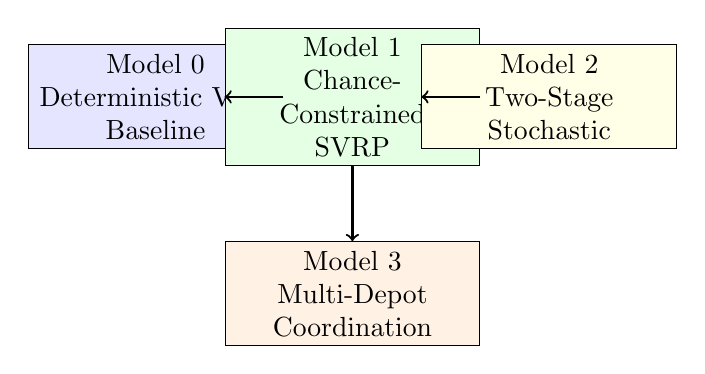
\begin{tikzpicture}[node distance=2.5cm,auto]
  \node (m0) [rectangle, draw, fill=blue!10, text width=3cm, align=center] {Model 0\\Deterministic VRP\\Baseline};
  \node (m1) [rectangle, draw, fill=green!10, text width=3cm, align=center, right of=m0] {Model 1\\Chance-Constrained\\SVRP};
  \node (m2) [rectangle, draw, fill=yellow!10, text width=3cm, align=center, right of=m1] {Model 2\\Two-Stage\\Stochastic};
  \node (m3) [rectangle, draw, fill=orange!10, text width=3cm, align=center, below of=m1] {Model 3\\Multi-Depot\\Coordination};

  \draw[->, thick] (m0) -- (m1);
  \draw[->, thick] (m1) -- (m2);
  \draw[->, thick] (m1) -- (m3);
\end{tikzpicture}
\caption{Model progression: from deterministic baseline to comprehensive stochastic framework}
\end{figure}

In Section \ref{sec:solution_algorithm}, we develop algorithms to solve these models for realistic problem instances.
